With the advent of cloud and multi-clouds a new vision of data integration is to be considered.
In this vision 
(i) \textit{data services} provide access and allow data retrieval;  
(ii) \textit{data processing services} retrieve and process data; 
(iii) \textit{data services} and \textit{data processing services} can be deployed in different \textit{cloud providers} geographically distributed; 
(iv) \textit{data services}, \textit{data processing services} and the \textit{cloud} itself export their SLA defining the services they provide and the quality conditions under which they are delivered. Different levels of SLA are considered: contracts agreed between \textit{data services} or \textit{data processing services} and \textit{cloud providers}, called \textit{cloud SLA} (SLA$_{C}$); and contracts agreed between users and \textit{data services} or \textit{data processing services}, called \textit{service SLA} (SLA$_{S}$). 
Therefore, given a user query, his/her integration quality requirements and his/her cloud subscription, the query is rewritten in terms of cloud services (\textit{data services} and \textit{data processing services}) composition that fulfill the integration requirements and deliver the expected results to the user.
%The figure~\ref{fig:scenario} illustrates our data integration vision.

% \begin{figure}[h!]
% \center
% 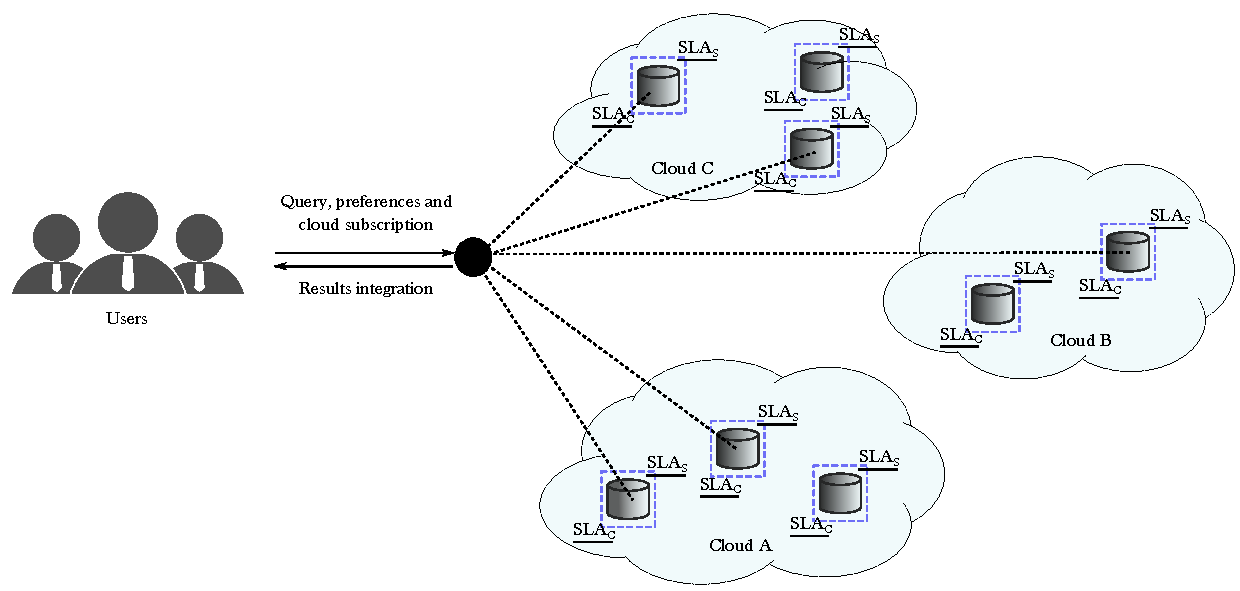
\includegraphics[scale=0.57]{scenario.pdf}
% \caption{New vision of data integration}\label{fig:scenario}
% \end{figure}

To better understand our vision and challenges, let us consider the following medical scenario in which users are able to retrieve and integrate data concerning (i) \textit{patients that were infected by a disease;}
(ii) \textit{regions most affected by a disease}; (iii) \textit{patients' personal information}; and (iv) \textit{patients' DNA information}. For instance, doctor \textit{Marcel} would like to study the type of people suffering of \textit{flu} in the Europe. To perform this, he has at his disposal a set of cloud services delivered by different \textit{cloud providers}.
Each cloud service and \textit{cloud provider} describe their quality guarantees in SLA contracts. Thereby, to reach his needs, he wants to query the personal and DNA information from patients infected by \textit{flu}, using cloud services with availability higher than 98\%, price per call less than 0.2\$ and integration total cost less than 5\$. This scenario introduces new challenges to data integration that have to be addressed, such as:
\begin{itemize}
\item Data integration tasks can require a huge amount of resources and processing time given the large quantity of \textit{data services} and \textit{data processing services};
\item The cloud model comes with the possibility of an on-demand and pay-per-use access to resources. However, cloud consumers have a restricted to the resources according to the contract they have with the cloud, and to the budget they are ready to pay while integrating data.
\item Part of the rewritings produced and executed to the user \textit{query} could not be in accordance with her quality requirements. In addition, generating these unsatisfactory rewritings imply increasing  the processing time and integration cost. Consequently, the user may become dissatisfied with the results. 
\item Performing data integration in this scenario implies a matching problem of users' requirements with different services' guarantees specified in SLAs. Considering the multi-cloud environment, we can face different cases of SLA incompatibilities given the different semantics and structure of SLAs exported by the different cloud services and \textit{cloud providers}.
\item Executing data integration tasks is computationally costly in terms of processing time and economic cost. Therefore, it is crucial to reuse previous integration results in order to save time and money while satisfying the user.
\end{itemize}

Motivated by the challenges discussed above, the figure~\ref{fig:workflow} illustrates our SLA-based data integration workflow. Given a user query, a set of user preferences associated to it, cloud providers and cloud services, the workflow can be divided in four steps:

\begin{figure}[h!]
\center
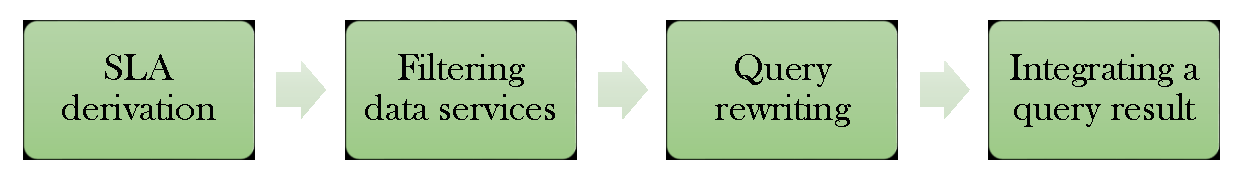
\includegraphics[scale=0.40]{workflow-approach.pdf}
\caption{SLA-based data integration workflow}\label{fig:workflow}
\end{figure}

\noindent \textbf{\underline{SLA derivation}}. In this step, we compute what we call a \textsl{derived SLA} that matches user' integration requirements (including quality constraints and data requirements) with the SLA's provided by \textit{cloud services}, given a specific user cloud subscription. The user may have general \textit{preferences} depending on the context he/she wants to integrate his/her data such as economic cost, bandwidth limit, free services, and storage and processing limits. The \textit{SLA derivation} is the big challenge while dealing with SLAs and particularly for adding quality dimensions to data integration. Furthermore, the \textsl{derived SLA} guides the query evaluation, and the way results are computed and delivered. \\
\textbf{\underline{Filtering data services}}. The \textsl{derived SLA} is used (i)
to filter previous \textsl{integration SLA} derived for a similar request in order to reuse results; or (ii) to filter possible \textit{cloud services} that can be used for answering the query. \\ %The SLA exported by a selected \textit{cloud service} should satisfy the user \textit{preferences}. \\
\textbf{\underline{Query rewriting}}. Given a set of \textit{data services} that can
potentially provide data for integrating the query result, a set of service compositions is generated according to the \textsl{derived SLA} and the agreed SLA of each \textit{data services}. \\
\textbf{\underline{Integrating a query result}}. The service compositions are
executed with services from one or several clouds where the user has a
subscription.
The execution cost of service compositions must fulfill the \textsl{derived
SLA}. The clouds resources needed by the user to execute the composition and how
to use them is decided taking in consideration the economic cost determined by
the data to be transferred, the number of external calls to services, data storage and delivery cost.

Although \textit{the SLA derivation} is the big challenge while dealing with
SLAs and particularly for adding quality dimensions to data integration, the
focus in this paper is our query rewriting algorithm which deals with user
preferences and SLAs exported by different cloud providers and data services.
Here, we are assuming that there is a mechanism responsible to extract the
services' quality aspects from SLA, and to provide this information as input to
the algorithm. The figure~\ref{fig:cloudsla} illustrates the structure of SLA
and its measures that are considered in the algorithm we will detail in the next
section.   

\begin{figure}[h!]
\center
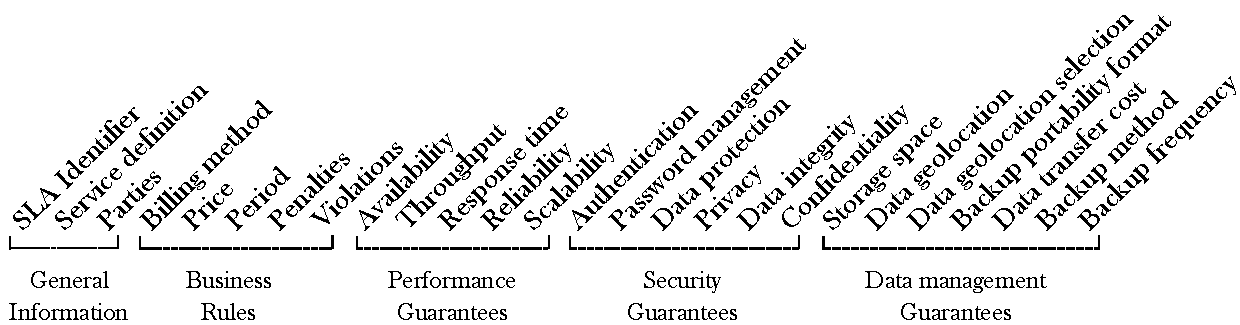
\includegraphics[scale=0.47]{Cloud_SLA.pdf}
\caption{Cloud SLA model}\label{fig:cloudsla}
\end{figure}